%-------------------------------------------------------------------------------
\chapter{Experiments and Results}
\labelchapter{ch.expe}
%-------------------------------------------------------------------------------

%%%%%%%%%%%%%%%%%%%%%%%%%%%%%%%%%%%%%%%%%%%%%%%%%%%%%%%%%%%%%%%%%%%%%%%%%%%%%%%%
%%%%%%%%%%%%%%%%%%%%%%%%%%%%%%%%%%%%%%%%%%%%%%%%%%%%%%%%%%%%%%%%%%%%%%%%%%%%%%%%

\lettrine[lines=2]{T}{his} chapter introduces the experiments that were run to demonstrate the usability of both the estimation and the exploration methodologies that were described in the previous chapters.

We built a \chisel-based demonstrator as a {\it proof of concept} framework, as well as a benchmark of representative applications for analysis and comparison purposes.
We then ran multiple experiments to exhibit how \myLongAcs{HCL}{Hardware Construction Language} can be used to improve the life of developers, with a particular focus on their usage for \myLongAc{DSE}{Design Space Exploration}.

\vspace*{\fill}
\minitoc 
\mtcskip 

\newpage
%%%%%%%%%%%%%%%%%%%%%%%%%%%%%%%%%%%%%%%%%%%%%%%%%%%%%%%%%%%%%%%%%%%%%%%%%%%%%%%%

% SECTION
\section{Building a Software Demonstrator}
\label{ch.expe:sec.qece}
    In order to demonstrate the usability of the methodologies introduced in Sections \ref{ch.estimators} and \ref{ch.dse}, we built a \chisel-based framework --- which is called \myLongAc{QECE}{Quick Exploration using Chisel Estimators} --- and integrated it into the \myLongAc{HCF}{Hardware Construction Framework}.

    \subsection{Implementation Details}
    \label{ch.expe:sec.qece:ssec.impl}

        \myAc{QECE} was built in a flexible and modular way, to allow users to easily define both custom estimators and exploration strategies.
        It leverages \scala{} high level features to use software methodologies in hardware design processes.
        
        \subsubsection{Meta design}
            To do so, the first step was to enable users to exploit the {\bf meta design methodology}, in order to expose the design space to be explored at module constructor level, as stated in Section \ref{ch.dse:sec.explorable:ssec.generators}.
            This was made possible by using the \java{} annotation system (as can be seen in Listing \ref{ch.dse:sec.explorable:ssec.generators:list.dotproduct} for example).
            We also added an annotation system to specify the impact of the parameters on given metrics, enabling to leverage the user knowledge at both implementation and exploration stages, by introducing a relationship between parameters and strategies.
            It is done by defining a new annotation class: \lstinline{class ImpactMetric(name: String) extends StaticAnnotation} --- where the \lstinline{name} parameter is used to identify a particular metric.\footnote{The \lstinline{@qualityOfService} annotation used in Listing \ref{ch.dse:sec.explorable:ssec.generators:list.dotproduct} is a simple alias for \lstinline{ImpactMetric("qualityOfService")}.}

        \subsubsection{Integrating estimators}
            In a second time, we developed wrappers around the \firrtl{} transforms to enable a seamless estimator integration, as exposed in Section \ref{ch.estimators:sec.integration:ssec.api}.

            We implemented both {\bf resource} and {\bf timing} estimators using linear interpolations and macro block replacements to allow an early estimation of the metrics in the exploration flows.

            Some empirical \myLongAc{QoS}{Quality of Service} estimators were implemented by binding to the \chisel{} simulation backends, as shown in Figure \ref{ch.estimators:sec.integration:ssec.multi-fidelity:fig.flow}.
            Doing so, one can retrieve some metrics from simulations, and can thus build their own test benches, defining both which metrics they want to get and how they are computed.
            As an example, we added helpers to compute the \myLongAcs{RMSE}{Root-Mean-Square Error} from the simulation results, by providing an initial workload and a software golden reference.

            Finally, we enabled building any {\bf analytical estimator} operating on pre-existing metrics in the flow --- users can thus easily define analytical formulas directly in their strategies.

        \subsubsection{Building strategies}
            We then built a flexible way to enable {\bf meta exploration} by implementing a generic \lstinline{Strategy} class, which can then be used to define more or less complex strategies, as defined in Section \ref{ch.dse:sec.functional}.

            \begin{figure}[h!]
                \centering
                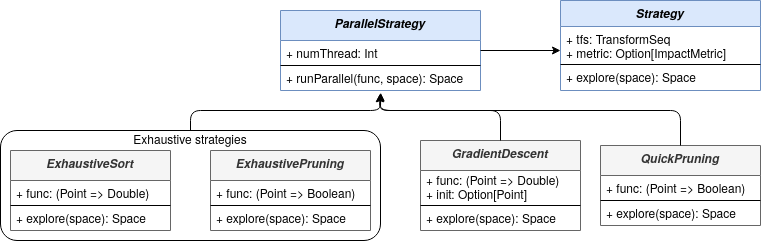
\includegraphics[width=1.0\textwidth]{Figures/Implementation-Strategies.png}
                \caption{Object hierarchy for the implemented strategies}
                \label{ch.expe:sec.qece:ssec.impl:fig.strategies}
            \end{figure}

            Figure \ref{ch.expe:sec.qece:ssec.impl:fig.strategies} introduces the different strategies that were built for this demonstrator, which have already been discussed in Section \ref{ch.dse:sec.functional:ssec.basic}.
            As we can see, every implemented strategy inherits from the base \lstinline{Strategy} class through \lstinline{ParallelStrategy}, as each can take advantage of parallel threads to speed-up the estimations.
            The strategies rely on custom defined parameters that allow the users to finely tune every step of the process --- it includes the {\bf estimation transforms} \lstinline{tfs} to be run, the {\bf number of parallel threads} available, or different ways to estimate and compare the explored implementations. 
            For both {\bf pruning strategies}, the users hence need to provide a {\bf boolean function} which specify if a point should be removed from the space, while the two other strategies rely on a {\bf cost function} which build a new metric from a set of existing ones.

            The \lstinline{ImpactMetrics} are considered at strategy level to reduce the design space dimension by removing the non impacting parameters if needed.
            The same mechanism is used for the dimension removal strategy that was exposed in Section \ref{ch.dse:sec.functional:ssec.basic}, in order to allow users to explicitly state that a given dimension will no more be relevant for the remaining of an exploration process.
            Moreover, as the introduced estimation processes are independent, we also implemented some helpers for parallelism exploitation in order to speed up the whole processes --- this is particularly helpful for time consuming estimation processes such as synthesis runs --- and we used caching techniques in the strategies to avoid multiple estimations of a same point. 
            We finally implemented composition and strategy building helpers as a syntactic sugar to enable straightforward strategy definitions in a functional fashion --- \ie the helpers hide all the side-effects needed for the strategy building, and expose the exploration processes as simple functions operating over spaces.

        \vspace{-0.15cm}
        \subsubsection{Design space implementation}
        \vspace{-0.05cm}
            Building custom exploration strategies is thus made possible in a expressive way.
            However, implementing a new strategy often relies on particular operations over the input space, implying that the data structure used for its implementation might have a huge impact on the exploration performances.

            In order to allow the users to define their own space structures, we propose a generic implementation for \lstinline{Spaces} in Figure \ref{ch.expe:sec.qece:ssec.impl:fig.space}, with the basic operations introduced in Section \ref{ch.dse:sec.functional} that are needed to explore them (\eg \lstinline{map}, \lstinline{filter} or \lstinline{getNeighbours} functions).
            It also includes operations to remove and add dimensions, for cases where the \lstinline{ImpactMetric}s are used to discriminate some dimensions in the current exploration.
            We use a hierarchical, object-oriented approach to allow the users to easily integrate their own space structures if needed.
            As each implementation defines its own operations, some spaces might be more suited for a given usage, and the strategy builder should choose a structure fitted for their need.
            For the needs of this demonstrator, we implemented two different structures: \lstinline{SeqSpaces} and \lstinline{MatrixSpaces}.

            A \lstinline{SeqSpace} is a simple space based on the \scala{} \lstinline{Seq} collections, that can be used for sort purposes as it exposes an ordered structure.
            However, finding the neighbourhood of a multidimensional \lstinline{Point} in a flatten representation of the space requires to scan it exhaustively, evaluating each distance and selecting only the nearest points.
            As a \lstinline{SeqSpace} does not exhibit any pattern to directly access to the neighbourhoods, exploring the neighbours of a \lstinline{Point} in a large space can thus result in an exploding complexity.

            On the other hand, a \lstinline{MatrixSpace} is based on the \scala{} representation of matrices, built on multidimensional \lstinline{Arrays}. 
            Each dimension of the space is represented at a different level in the built {\bf hyper matrix}, and the space also includes a dictionary mapping each dimension to all the possible values.
            This enables to easily define the neighbourhood of a point, with a complexity growing linear with the different dimensions of the space (which is ideal to define efficient {\bf gradient descent based strategies}).
            This also means that the matrices may be sparse, for points that have already been pruned.
            However, such \lstinline{Space} cannot be sorted as the structure does not exhibit an order, and the \scala{} \lstinline{Array}-based implementations can only be used for dimensions ranging from 1 to 5 --- which is a limitation of the language --- even if adding dimensions is possible in a custom way if needed.

\clearpage
            \begin{figure}[h!]
                \centering
                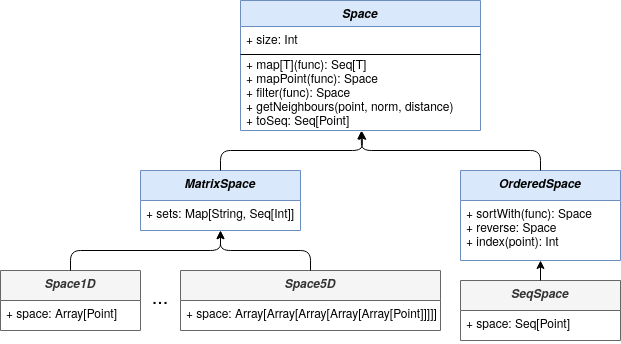
\includegraphics[width=1.0\textwidth]{Figures/Implementation-Space.png}
                \caption{Proposing different space implementations}
                \label{ch.expe:sec.qece:ssec.impl:fig.space}
            \end{figure}

        \subsubsection{A functional demonstrator}
            Using those two space implementations and the five basic strategies introduced in Chapter \ref{ch.dse}, we built \myAc{QECE} as a {\it proof of concept} framework that will be used to demonstrate the advantages of the proposed methodologies.

            We deliver \myAc{QECE} as an open-source solution, to enable using the introduced methodologies in any \chisel-based project \cite{ferres_qece_2021}.

    \subsection{Use Case: Exploring GEMM Implementations}
    \label{ch.expe:sec.qece:ssec.usecase}

            We introduce a (simplified) example of the usage of \myAc{QECE} for a {\bf gradient descent based exploration} on \myLongAc{GEMM}{General Matrix Multiply} kernels in Listing \ref{ch.expe:sec.qece:list.gradient}, implementing the strategy exposed in Figure \ref{ch.dse:sec.functional:ssec.complex:fig.complex:sfig.gradient}.

            For each strategy, the user needs to define the set of {\bf estimation transforms} \lstinline{tfs} to be run, and some functions to specify the exploration behaviour:%
            \footnote{ The \lstinline{++} operation is used to build an ordered set of {\bf estimation transforms}.} %
            for both \lstinline{sort} and \lstinline{gradient} steps, he needs to provide a function \lstinline{func} to associate a cost to each implementation, as well as a comparison function \lstinline{cmp} to expose an order relationship, while the \lstinline{prune} step only requires a boolean function (also called \lstinline{func}) to specify whether a point is to be removed or to be kept in the resulting design space.

            The different metrics at stake in this use case are \lstinline{%lut}, \lstinline{%dsp} and \lstinline{throughput}, which respectively corresponds to the usage of \myAcs{LUT} and \myAcs{DSP}, and to the theoretical throughput of the considered implementations.

            The defined strategy is based on three consecutive steps:
            \begin{enumerate}
                \item {\bf lines 2-5:} Estimate the resource usages and {\bf prune the implementations} that consume {\bf too many resources}.\footnote{Thresholds are arbitrary and shall depend on the accuracy of the used estimators.}
                \item {\bf lines 7-10:} Sort the design space to {\bf select the widest implementation} that still fits on the target board, after this first pruning.
                \item {\bf lines 12-17:} Use this implementation as the starting point of a {\bf gradient descent algorithm} based on synthesis runs, aiming to find local optimum in an already pruned space (using the {\bf throughput (GOp/s)} as the objective function to optimize).
            \end{enumerate}

            As the \myAc{GEMM} algorithm is computation intensive, we chose to consider only the \myLongAcs{LUT}{Look-Up Table} and \myLongAcs{DSP}{Digital Signal Processor} usages for step 1., as the wide implementations will probably saturate the available \myAcs{LUT}/\myAcs{DSP} before the other resources --- it is important to note that this decision is based on our expertise about hardware design.
            For step 2., we then chose to define the {\bf widest design} as the implementation estimated to consume the greatest amount of \myAcs{LUT} for similar reasons, with the hypothesis that the implementation with the maximal throughput --- but that still fits on the target board --- will be near this estimated widest implementation.
            This is then used in step 3., as the gradient strategy will use the first point of the sorted space as the starting point for the descent.
            We thus improve the convergence speed as we know that the implementations where both \myAcs{LUT} and \myAcs{DSP} are estimated to be low will probably not be the optimal ones.

            We defined some aliases for the estimation transforms to be run, to keep the strategy concise and intelligible:
            \begin{itemize}
                \item \lstinline{TransformSeq.resources} performs a \firrtl{} estimation of the circuit resource usage, using the methodology introduced in Section \ref{ch.estimators:sec.resource-timing}.
                \item \lstinline{TransformSeq.synthesis} runs a synthesis backend and performs a report analysis to provide both resource usage and operating frequency.
                \item \lstinline{TransformSeq.throughput} computes the throughput using an analytical formula (Eq. \ref{app.benchmark:sec.gemm:eq.throughput}).
                    The implementations that did not fit on the target board after the synthesis are marked as having a null throughput.
            \end{itemize}

\clearpage
            Using those transforms, we can express the exploration flow schematized in Figure \ref{ch.dse:sec.functional:ssec.complex:fig.complex:sfig.gradient} in a readable, intelligible manner, by composing exploration steps in a functional fashion.
            Each exploration step --- \ie \lstinline{prune}, \lstinline{sort} and \lstinline{gradient} --- corresponds to a \lstinline{Strategy} as defined in Section \ref{ch.expe:sec.qece:ssec.impl}, defining the estimation transforms to be run and the \lstinline{Space} operations to be performed, resulting in a complex, application specific strategy.


        \begin{figure}[h!]
            \begin{lstlisting}[caption={[Gradient based strategy definition]Defining a gradient descent based strategy (Fig. \ref{ch.dse:sec.functional:ssec.complex:fig.complex:sfig.gradient}) in QECE},
                               label={ch.expe:sec.qece:list.gradient}]
explore(
    // prune the designs using too much DSP/LUT
    prune(
        tfs  = TransformSeq.resources,
        func = (%dsp > x || %lut > y)
    ),
    // select the widest design to start descent
    sort(
        func = %lut,
        cmp  = (\_ > \_)
    ),
    // use gradient descent for exploration
    gradient(
        tfs  = TransformSeq.synthesis ++ 
               TransformSeq.throughput,
        func  = throughput,
        cmp   = (\_ > \_)
    )
)\end{lstlisting}
        \end{figure}

%%%%%%%%%%%%%%%%%%%%%%%%%%%%%%%%%%%%%%%%%%%%%%%%%%%%%%%%%%%%%%%%%%%%%%%%%%%%%%%%%

% SECTION
\section{Application Benchmark}
\label{ch.expe:sec.benchmark}

    To demonstrate how \myAc{QECE} can be used to improve the developer productivity, we built an open-source benchmark of digital applications that are relevant for \myAc{FPGA}-based implementations \cite{ferres_benchmark_2021}.

    Appendix \ref{app.benchmark} exposes how the {\bf meta design} methodology has been applied to each kernel of the benchmark.
    More specifically, Table \ref{app.benchmark:table.benchmark} introduces its composition as well as all the exposed design spaces.
    
%%%%%%%%%%%%%%%%%%%%%%%%%%%%%%%%%%%%%%%%%%%%%%%%%%%%%%%%%%%%%%%%%%%%%%%%%%%%%%%%%

% SECTION
\section{Experimental Setups}
\label{ch.expe:sec.setup}

    The experiments were run on two different experimental setups, as two servers were available.
    Their characteristics are introduced in Table \ref{ch.expe:sec.setup:table.setup}.

    \begin{table}[h!]
        \centering
        \begin{tabular}{cccccc}
            {\bf Name} & {\bf Mark} & {\bf\#Core} & {\bf Frequency} & {\bf RAM} & {\bf Vivado} \\
            \hline
            Server 1 & \pomahaka & 12 & 3.46 GHz & 78.8 GB & v2017.3\\
            \ccg Server 2 & \ccg\styx & \ccg 24 & \ccg 3.2 GHz & \ccg 188 GB & \ccg v2021.1\\
        \end{tabular}
        \caption{Experimental setups characteristics}
        \label{ch.expe:sec.setup:table.setup}
        \vspace{-0.4cm}
    \end{table}

    It is important to note that \vivado{} specifications claims that at most {\bf 8 GB} of \myAc{RAM} will be used when targeting a \VC{} board \cite{xilinx_memory_2021}.
    % It is important to note that \vivado{} memory usage specifications claims that at most {\bf 8 GB} will be used when targeting a \VC{} board \cite{xilinx_memory_2021}.
    However, the memory consumption is given only for designs that consume $\approx 80\%$ of the available resources --- meaning that, for wider designs, the memory usage may explode.
    To cope with this problem, we had to define a {\bf 2-hours synthesis timeout}, in order to keep the memory usage under constraint and avoid crashes.
    We empirically noticed that doing so keeps the memory usage under 20 GB for each synthesis, meaning that we can respectively run at most 4 and 9 synthesis at once on server 1 and 2.
    As the version of \vivado{} can lead to different implementation choices, it is important to consider which version of the software suite was used for syntheses --- it is also important to note that given the version and/or the synthesis heuristics used, synthesis results may vary a lot: the whole flow is highly dependent on the quality of the synthesis software used.

    For the next sections, please refer to the column {\bf Mark} to know which setup was used for a particular experiment.

%%%%%%%%%%%%%%%%%%%%%%%%%%%%%%%%%%%%%%%%%%%%%%%%%%%%%%%%%%%%%%%%%%%%%%%%%%%%%%%%%

% SECTION
\section{Quality of the Estimators}
\label{ch.expe:sec.estimators}

    In this section, we will discuss the quality of the estimation methodologies that were defined in Chapter \ref{ch.estimators}, and show that our demonstrator is able to leverage imperfect yet exploitable estimators for both resource and \myAc{QoS} metrics.
    We will also tackle the usability of our approach for timing estimation, as well as limitations of such approach in quick exploration processes.

    \subsection{Resource Estimations}
    \label{ch.expe:sec.estimators:ssec.resource}

        Figure \ref{ch.expe:sec.estimators:ssec.resource:fig.all} introduces a measure of the \myLongAc{QoR}{Quality of Results} of the {\bf graph level resource estimators} --- or \firrtl-based estimators --- that were described in Section \ref{ch.estimators:sec.resource-timing}.
        The \myAc{QoR} is computed with respect to the synthesis results for 5 different {\bf meta designs} (see Table \ref{ch.expe:sec.estimators:ssec.resource:table.kernels}).

        For each implementation, we ran three types of resource estimators:%
        \footnote{To keep both resource usage and processing time acceptable, we set a {\bf 30 minute timeout} for both macro replacement and resource usage estimation transforms.}
        \begin{enumerate}
            \setlength\itemsep{-.3em}
            \item \firrtl-based estimation, without macro block (see Section \ref{ch.estimators:sec.resource-timing:ssec.basic})
            \item \firrtl-based estimation, using macro blocks (see Section \ref{ch.estimators:sec.resource-timing:ssec.macro})
            \item {\bf Synthesis} based estimation, used as baseline (\ie reference value)
        \end{enumerate}

        We then plotted the relative difference histograms of both estimations 1. and 2. with respect to 3., respectively in Figures \ref{ch.expe:sec.estimators:ssec.resource:fig.all:sfig.without} and \ref{ch.expe:sec.estimators:ssec.resource:fig.all:sfig.with}, to analyse the \myAc{QoR} of both estimation methodologies.
        To do so, for each implementation of each kernel, we tried to run those three estimators, computed the relative differences with respect to the synthesis results, and built relative difference classes for each resource type (\myAcs{LUT}, \myAcs{FF}, \myAcs{DSP} and \myAcs{BRAM}).
        Those classes were then plotted in order to exhibit the impact of each estimation methodology, for all the considered resources.
        
        \begin{figure}[h!]
            \vspace{-0.2cm}
            \centering
            \begin{subfigure}{1.0\textwidth}
                \centering
                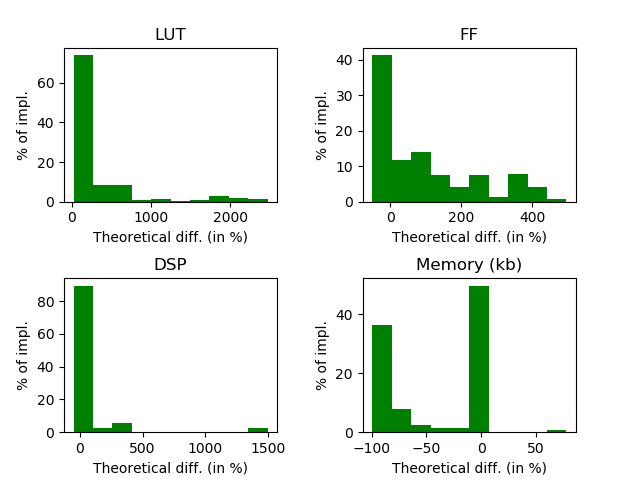
\includegraphics[width=0.83\textwidth]{Figures/results/allRelativeWithoutMacro}
                \caption{Resource estimation (without macro block replacement)}
                \label{ch.expe:sec.estimators:ssec.resource:fig.all:sfig.without}
            \end{subfigure}
            \begin{subfigure}{1.0\textwidth}
                \centering
                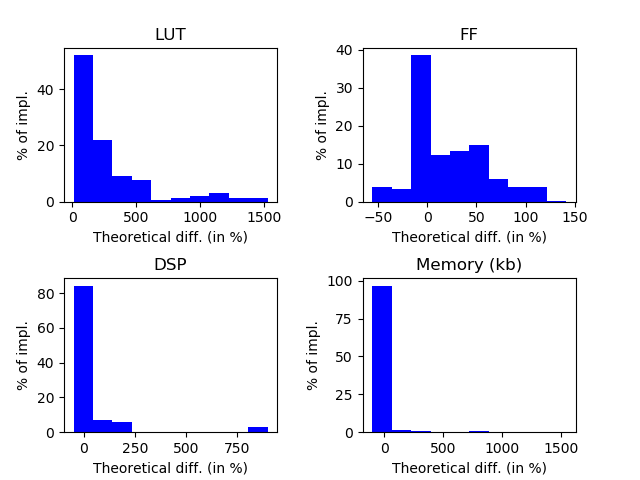
\includegraphics[width=0.83\textwidth]{Figures/results/allRelativeWithMacro}
                \caption{Resource estimation (with macro block replacement)}
                \label{ch.expe:sec.estimators:ssec.resource:fig.all:sfig.with}
            \end{subfigure}
            \caption[Quality of resource estimations on various kernels]{Average relative differences on 5 different {\bf meta designs} between the resource estimations and the synthesis results.\textsuperscript{\styx}\newline The kernels are introduced in Table \ref{ch.expe:sec.estimators:ssec.resource:table.kernels}.}
            \label{ch.expe:sec.estimators:ssec.resource:fig.all}
        \end{figure}

        \renewcommand*{\thefootnote}{\fnsymbol{footnote}}
        \begin{table}[h!]
            \scalebox{0.9}{
                \begin{tabular}{cccccc}
                    \multirow{2}*{{\bf Kernel}} & \multirow{2}*{{\bf Space}} & {\bf Estimations} & \multicolumn{3}{c}{{\bf Estimation time}} \\
                    ~ & ~ & {\bf ({\it failures})} & Synthesis &  Macro & No macro\\
                    \hline
                    \myAc{GEMM}\footnotemark[9] & 168 & 151 (46) & 15h48m11s & 2h00m42s & 25m55s \\
                    \ccg Black Scholes\footnotemark[9] & \ccg 162 & \ccg 42 (3) & \ccg 2h57m16s & \ccg 10m19s & \ccg 8m12s \\
                    Pi\footnotemark[9] & 162 & 90 (12) & 39m50s & 4m14s & 1m05s \\
                    \ccg \myAc{FFT}\footnotemark[9] & \ccg 200 & \ccg 173 (22) & \ccg 9h51m16s & \ccg 3h14m06s & \ccg 2h14m37s\\
                    Dot product\footnotemark[9] & 144 & 144 (0) & 27m54s & 29s & 26s \\
                    \hline
                    \hline
                    {\bf Total} & {\bf 836} & {\bf 600 (83)} & {\bf 29h44m27s} & {\bf 5h59m50s} & {\bf 2h50m15s}\\
                \end{tabular}
            }
            \caption[Temporal behaviour of resource estimators]{Design spaces and running times of resource estimators (Fig. \ref{ch.expe:sec.estimators:ssec.resource:fig.all})}
            \label{ch.expe:sec.estimators:ssec.resource:table.kernels}
        \end{table}
        \renewcommand*{\thefootnote}{\arabic{footnote}}

        We observe that using the naive approach --- \ie without macro block replacement (Fig. \ref{ch.expe:sec.estimators:ssec.resource:fig.all:sfig.without}) --- the estimation accuracy is quite variable:
        \begin{itemize}
            \item the \myAcs{LUT} are estimated within $[\![0\%, 1000\%]\!]$ of the real usage for more than 80\% of the considered designs
            \item the \myAcs{FF} are estimated within $[\![0\%, 400\%]\!]$ of the real usage, and even under 200\% for a majority of designs
            \item the \myAcs{DSP} are almost always estimated perfectly, but errors in the estimations may result in a 1500\% overestimation
            \item the \myAcs{BRAM} are estimated within $[\![-100\%, 100\%]\!]$ of the real usage, and are perfectly estimated for a majority of designs
        \end{itemize}

\clearpage
        Based on the Figure \ref{ch.expe:sec.estimators:ssec.resource:fig.all:sfig.with}, we can then remark that using macro block replacements has a big impact on the estimations \myAc{QoR}.
        The \myAc{LUT} estimations are now mainly produced in a $[\![0\%, 500\%]\!]$ interval, while the \myAc{FF} estimations are now estimated within $[\![-50\%, 100\%]$.
        The \myAc{DSP} estimations are mainly as good as with the naive version, but extrema are divided by a factor 2, and the \myAc{BRAM} usage is now always perfectly estimated.

        We can thus claim that those estimators are not perfect, and that the estimation variability could be considered too big to be exploitable.
        However, some tendencies can be exhibited here, that could be used to take decisions based on the estimations only:
        \begin{itemize}
            \item for most designs, using a factor 6 on the \myAc{LUT} estimation can enable to estimate whether a design fits on the target board or not
            \item similarly, using a factor 2 for \myAcs{FF} can lead to realistic decisions
            \item both \myAc{DSP} and \myAc{BRAM} estimations can be trusted for most designs
        \end{itemize}

        As for the estimation process speed, we can observe in Table \ref{ch.expe:sec.estimators:ssec.resource:table.kernels} that both the naive and the macro based approaches are way faster than synthesis runs, which was the main objective of those techniques.
        We can also remark that using the macro block replacement methodology can consume a lot more time that the naive approach, and it is specifically true for large and complex designs such as \myAc{GEMM} or \myAc{FFT}.
        It is actually due to the implementation of the macro replacement technique, which is based on building another graph from the \myAc{FIRRTL} representation, and which does not seem to scale on large designs.
        Most of the time is due to timeouts of the graph building processes, and this could be mitigated by using a more optimized technique to do so.

        We thus showed that the graph level techniques that were introduced in Chapter \ref{ch.estimators} can be used to perform an early resource estimation, and could be leveraged for early decision making from the developers.        
        However, we still need to exhibit what impact it can have on those decisions, and it will be discussed later in this chapter.

        \subsubsection*{Remark}
        While we did exhibit the \myAc{QoR} of the estimation methodologies on 5 different {\bf meta designs}, one may want to analyse the quality of both methodologies for a particular kernel. 
        For this purpose, we expose a disaggregated version of Figure \ref{ch.expe:sec.estimators:ssec.resource:fig.all} in Appendix \ref{app.resource} --- except for the \myAc{GEMM} kernels, which results are exposed in Figure \ref{ch.expe:sec.strategies:ssec.resource:fig.gemm} as they will be used in later experiments.

    \subsection{Timing Estimations}
    \label{ch.expe:sec.estimators:ssec.timing}

       As for the timing estimations, Figure \ref{ch.expe:sec.strategies:ssec.timing:fig.gemm} introduces some considerations on both the estimation processing times and the \myAc{QoR} for \myAc{GEMM} kernels, with respect to the synthesis results.
       Table \ref{ch.expe:sec.estimators:ssec.timing:table.gemm} provides more information about the explored design space and the temporal behaviour of these experiments.%
       \footnote{For the naive approach --- \ie without macro block replacement --- the timing estimations are not fully available, as the memory blocks cannot properly be estimated.
       However, the path building algorithm was run anyway to estimate the processing time.}

        \begin{table}[h!]
            \scalebox{0.9}{
                \begin{tabular}{c|cccc}
                    \multirow{2}*{{\bf Space size}} & \multirow{2}*{{\bf Estimator}} & {\bf Successful} & \multirow{2}*{{\bf Timeouts}} & \multirow{2}*{{\bf Exploration time}} \\ 
                    ~ & ~ & {\bf estimations} & ~ & ~ \\
                    \hline
                    \multirow{5}*{168} & Synthesis & 102 & 49 & 15h48m24s\\
                    ~ & \ccg RTL estimation & \ccg ~ & \ccg ~ & \ccg ~\\
                    ~ & \ccg (with macro) & \multirow{-2}*{\ccg 94} & \multirow{-2}*{\ccg 57} & \multirow{-2}*{\ccg 11h20m15s}\\
                    ~ & {\it RTL estimation} & ~ & ~ & ~\\
                    ~ & {\it (without macro)} & \multirow{-2}*{-} & \multirow{-2}*{-} & \multirow{-2}*{{\it $\approx$8h}}\\
                \end{tabular}
            }
            \caption[Timing estimations over GEMM implementations]{Timing estimations over GEMM\textsuperscript{\styx} implementations (Fig. \ref{ch.expe:sec.strategies:ssec.timing:fig.gemm})}
            \label{ch.expe:sec.estimators:ssec.timing:table.gemm}
        \end{table}

       For those experiments, a {\bf 2 hours timeout} was used for both macro replacement and critical path estimation transforms, in order to keep the memory usage under constraints and avoid time consuming processes.
       Doing so, we remark that for both timing estimation approaches --- \ie with and without macro block replacement --- the estimation time is mostly kept way under the synthesis time.
       However, for complex designs, it can be longer than the synthesis.
       This is mainly due to the complexity of the path building algorithm, which unrolls every possible path on the considered design, and is thus similar to the synthesis process --- hence, it cannot be considered as a faster approach, as the algorithmic complexities are comparable.

        \begin{figure}[h!]
            \centering
            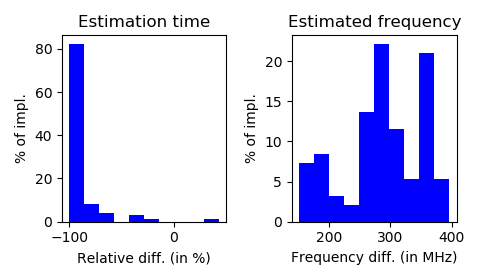
\includegraphics[width=1.0\textwidth]{Figures/results/gemmTimingWithMacro}
            \caption[Quality of frequency estimations on GEMM]{Relative difference between frequency estimations and synthesis\newline results on GEMM {\bf meta design}\textsuperscript{\styx} ({\it using macro block replacement})}
            \label{ch.expe:sec.strategies:ssec.timing:fig.gemm}
        \end{figure}

       Using only those considerations, we can already state that those approaches cannot be leveraged to build efficient design processes, as for more complex designs, actually synthesizing the circuit will result in a faster feedback for the users.
       Moreover, we can also remark that the frequency estimation is totally unrealistic, with differences of hundred of MHz between the estimations and the synthesis results.
        
       Based on those results, we consider this timing estimation methodology to be unpracticable with both approaches, and will not consider those estimators to be usable in the rest of this work.
       However, some methods exist to provide more realistic estimations of the operating frequency \cite{kwon_transfer_2020}\cite{paletti_dovado_2021}, and integrating them in \myAc{QECE} is considered, as they could bring both fast and interesting feedbacks to users and tools.

    \subsection{Quality of Service Estimations}
    \label{ch.expe:sec.estimators:ssec.qos}

        In order to estimate the \myAc{QoS} of a design, we propose an \myLongAc{API}{Application Programming Interface} to users in order to extract custom defined results from a simulation backend, as specified in Section \ref{ch.expe:sec.qece:ssec.impl}.
        To define an estimator, one needs to provide a {\bf simulation test bench} as well as a way to compute and extract the \myAc{QoS} of the design with respect to a given workload.% providing a generic way to define any empirical metric.

        Figure \ref{ch.expe:sec.estimators:ssec.qos:fig.qos} introduces a simple use case on the {\bf dot product} kernel, using \myAc{RMSE} as an error metric.
        We here provide a simple analysis of the impact of the data representation on the result of a dot product, and display the error rate, showing that integrating a custom defined \myAc{QoS} metric is possible in \myAc{QECE}.
        To define the data representation, we use a fixed point format and consider two parameters: the number of bits used for the {\it dynamic} (\ie the number of bits before the binary point), and the number of {\it precision} bits (\ie after the binary point).
        As the {\it parallelism level} does not impact the \myAc{QoS}, this dimension is not considered, while the number of elements by input vector is fixed to 8, for visualization purposes.

\clearpage
        \begin{figure}[h!]
            \centering
            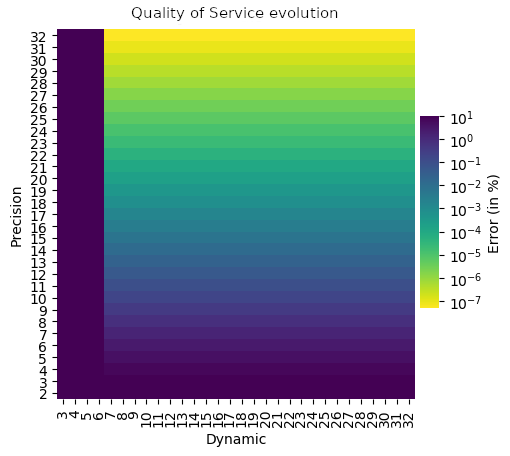
\includegraphics[width=1.0\textwidth]{Figures/results/qosEstimation.png}
            \caption[Quality of Service estimations on dot product]{Heatmap of the Quality of Service estimations for the dot\newline product {\bf meta design}\textsuperscript{\styx} ({\it vector size is fixed to 8 elements})}
            \label{ch.expe:sec.estimators:ssec.qos:fig.qos}
        \end{figure}

        The empirical approach for this estimator is based on comparing the simulation results with a software version of the same algorithm, based on a floating-point representation.
        Doing so, we can select only the designs which do not introduce a significant error in their results --- on this use case, it actually enables to compare the different data representations to select the ones sufficiently wide to absorb the errors that are induced by the use of a simpler representation.
        As the hardware implementation of \myLongAcs{FPU}{Floating-Point Unit} requires a lot of resources and time, such approach can be used to select a more efficient way to implement an algorithm, if the users can precisely state which error rates are acceptable.

\clearpage
        As can be seen on the heatmap, the implementations that use not enough {\it dynamic} bits are marked with a 10\% error rate, as representation overflows occurred during the simulations, resulting in a large error.%
        \footnote{The error rate introduced in Fig. \ref{ch.expe:sec.estimators:ssec.qos:fig.qos} is capped at 10\% and uses a logarithmic scale to properly visualize the smaller error rates, which are the region of interests in such explorations, as the acceptable error rate should be under 10\% to be meaningful.}
        Moreover, we can also observe the impact of the {\it precision} parameter on the \myAc{QoS}, from large representations where the error rate is under $10^{-7}\%$ to more compact ones, where the error rate reaches 10\%.

        While this use case is quite simple, it demonstrates that one can easily integrate an empirical, application specific estimator to estimate the \myAc{QoS} of its circuits, providing him with an interesting feedback that can be leveraged to select the best implementation that satisfy its accuracy need.

        For example, in Figure \ref{ch.expe:sec.estimators:ssec.qos:fig.qos}, we can (visually) state that if the applicative needs require an error rate lesser than 0.1\%, any implementation with more than 6 bits of {\it dynamic} and 10 bits of {\it precision} is enough.
    
%%%%%%%%%%%%%%%%%%%%%%%%%%%%%%%%%%%%%%%%%%%%%%%%%%%%%%%%%%%%%%%%%%%%%%%%%%%%%%%%%

\section{Comparing the Exploration Strategies}
\label{ch.expe:sec.strategies}
    We will now discuss how the user expertise can be leveraged for an efficient \myAc{DSE} definition, using the methodologies introduced in Chapter \ref{ch.dse}.

    For each strategy that will be compared in this section, the strategy definition is based on assumptions on both considered algorithm and target board, as our approach is based on providing users with ways to exploit their expertise instead of trying to define generic strategies for every algorithm.

    \subsection{Resource Estimation and Convergence Speed}
    \label{ch.expe:sec.strategies:ssec.resource}
    
        In a first time, we want to demonstrate how high level estimations of the resource usage can be used for the quicker convergence of an exploration strategy.
        We consider the exploration of two different {\bf meta designs} --- \myAc{FFT} and \myAc{GEMM} --- and compare the three exploration strategies that were introduced in Figure \ref{ch.dse:sec.functional:ssec.complex:fig.complex}.
        The results are exposed in Table \ref{ch.expe:sec.strategies:ssec.resources:table.explo}.
        For those experiments, the \myAc{QoS} is not considered, hence the element width is fixed by the developer (assuming that they can specify at exploration time that the chosen data representation is acceptable for the given use case), meaning that the {\it bit width} dimension is not considered in those explorations.

\clearpage
        \begin{table}[ht!]
            \centering
            \scalebox{0.68}{
                \centering
                \begin{tabular}{|c|c|c|c|c|c|c|c|}
                    \hline
                    \multirow{2}*{\bf Kernel} & \multirow{2}*{\bf Strategy} & \multirow{2}*{\bf Best throughput} & \multirow{2}*{\bf \#(space)} & {\bf \#synth} & \multirow{2}*{\bf Time} & \multirow{2}*{\bf Speed-up} \\
                    ~ & ~ & ~ & ~ & (\#timeout) & ~ & ~ \\
                    \hline
                    \multirow{3}*{\myAc{FFT}128\textsuperscript{\pomahaka}} & {\it Exhaustive} (Fig. \ref{ch.dse:sec.functional:ssec.complex:fig.complex:sfig.exhaustive}) & {\it 1.767 Tb/s} & \multirow{3}*{7} & {\it 7 (0)} & {\it 00h22m45s} & - \\
                    ~ & Pruning (Fig. \ref{ch.dse:sec.functional:ssec.complex:fig.complex:sfig.pruning}) & 1.767 Tb/s & ~ & 7 (0) & 00h24m14s & \inred{$\times$0.94} \\
                    ~ & Gradient (Fig. \ref{ch.dse:sec.functional:ssec.complex:fig.complex:sfig.gradient}) & 1.767 Tb/s & ~ & 3 (0) & 00h19m51s & $\times$1.15 \\
                    \hline
                    \multirow{3}*{\myAc{FFT}512\textsuperscript{\pomahaka}} & {\it Exhaustive} & {\it 5.479 Tb/s} & \multirow{3}*{9} & {\it 9 (0)} & {\it 02h11m51s} & - \\
                    ~ & Pruning & 5.479 Tb/s & ~ & 9 (0) & 03h17m52s & \inred{$\times$0.66} \\
                    ~ & Gradient & 5.479 Tb/s & ~ & 3 (0) & 02h18m29s & \inred{$\times$0.95} \\
                    \hline
                    \multirow{3}*{\myAc{GEMM}\textsuperscript{\pomahaka}} & {\it Exhaustive} & {\it 231.334 GOp/s} & \multirow{3}*{41} & {\it 41 (19)} & {\it 13h51m56s} & - \\
                    ~ & Pruning &  231.334 GOp/s & ~ & 26 (7) & 08h52m00s & $\times$1.5 \\
                    ~ & Gradient & 231.334 GOp/s & ~ & 6 (1) & 03h21m06s & $\times$4.1 \\
                    \hline
                \end{tabular}
                }
                \caption[Strategy comparison with no QoS concerns]{Comparing different exploration strategies with no quality of service concerns. {\it (Exhaustive strategies are used as baselines)}}
                \label{ch.expe:sec.strategies:ssec.resources:table.explo}
        \end{table}
\vspace{-0.6cm}
        \subsubsection{Defining a pruning function}

            For both kernels, we used a simple hypothesis to define the pruning function:
            \hyp{ch.expe:sec.strategies:ssec.resources:hyp.pruning}{Both FFT and GEMM kernels are computation intensive.}
            This means that the computational resources --- \ie \myAcs{LUT} and \myAcs{DSP} --- will be saturated first by the synthesis tool, and that removing too wide designs can be done by considering only those metrics.

            We thus defined the following {\bf pruning function} to be applied in both {\bf pruning} and {\bf gradient} strategies:
            \begin{equation}
                \label{ch.expe:sec.strategies:ssec.resource:eq.pruning}
                prune_{est.}(p) = LUT_{est.}(p) > 200\% \vee DSP_{est.}(p) > 100\%
            \end{equation}
            The thresholds were chosen with respect to the considerations that were discussed in Section \ref{ch.expe:sec.estimators:ssec.resource} and to the \myAc{QoR} of the resource estimations on \myAc{GEMM} kernels, as presented in Figure \ref{ch.expe:sec.strategies:ssec.resource:fig.gemm:sfig.with}.

            \subsubsection{Exploring {\it Fast Fourier Transform} implementations}

                For the \myAc{FFT} explorations, the design spaces are reduced as the size of the algorithm (see Table \ref{app.benchmark:table.benchmark} for the instantiation parameters) is considered fixed by the developers at exploration time --- meaning that \myAc{FFT} implementations of different sizes are not compared during the exploration processes.
                This results in a single dimension exploration space to be explored, for each possible \myAc{FFT} size.
                We only considered two different sizes --- 128 and 512 --- and we remark that for both explorations, the {\bf pruning strategy} is slower than the baseline, as no actual pruning is done in the design space.
                In fact, we actually applied the exhaustive strategy after running resource estimations, resulting in a consequent overhead with respect to the baseline.

                On the other hand, we remark that the {\bf gradient strategy} results in less synthesis needs for the same best fit finding --- meaning that even if the exploration time is not much impacted by the strategy choice, we can reduce the global processor time needed for parallel syntheses.
                In fact, for the \myAc{FFT}512, the actual convergence time is biased by synthesis timeouts, meaning that improving the resource estimators could enable to prune more efficiently the design space, and could help us avoiding long and non converging syntheses.% in the process.

                These use cases can be used to discuss the importance of the adequacy between the chosen exploration strategy and the explored kernel.
                Indeed, applying a preliminary pruning function to those use cases is not useful to speed-up explorations, and just results in a useless time overhead, while the gradient approach is practical and results in a speed-up that compensates that overhead.

            \subsubsection{Exploring {\it General Matrix Multiply} implementations}

            \begin{figure}[h!]
            \centering
            \begin{subfigure}{1.0\textwidth}
                \centering
                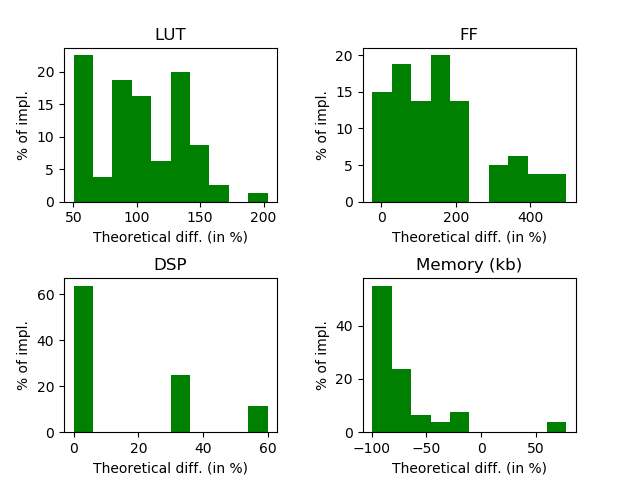
\includegraphics[width=0.85\textwidth]{Figures/results/gemmRelativeWithoutMacro}
                \caption{Resource estimation (without macro block replacement)}
                \label{ch.expe:sec.strategies:ssec.resource:fig.gemm:sfig.without}
            \end{subfigure}
            \begin{subfigure}{1.0\textwidth}
                \centering
                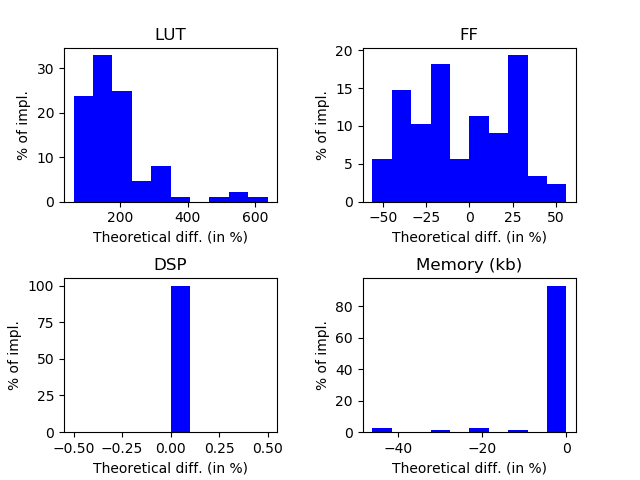
\includegraphics[width=0.85\textwidth]{Figures/results/gemmRelativeWithMacro}
                \caption{Resource estimation (with macro block replacement)}
                \label{ch.expe:sec.strategies:ssec.resource:fig.gemm:sfig.with}
            \end{subfigure}
            \caption[Quality of resource estimations on GEMM]{Relative difference between resource estimations and synthesis\newline results on GEMM implementations\textsuperscript{\styx}}
            \label{ch.expe:sec.strategies:ssec.resource:fig.gemm}
        \end{figure}

                For the \myAc{GEMM}-based explorations, we assumed that the defined pruning function (Eq. \ref{ch.expe:sec.strategies:ssec.resource:eq.pruning}) is more relevant, as it is based on an analysis of the \myAc{QoR} of the estimators on the \myAc{GEMM} implementations.
                We observe that applying this pruning function enables to reduce the number of implementations to be synthesized in the {\bf pruning strategy} by more than a third.
                More importantly, it reduces the number of synthesis timeouts by more than a half, as some non fitting designs that would cause long or non converging synthesis processes are not considered in this approach.

                In addition to this, we observe that using the {\bf gradient strategy} --- \ie leveraging both high level resource estimations and clever space traversal --- results in $\times 6.8$ less synthesis runs (6 instead of 41) and a $\times 4.1$ exploration speed-up.

                We thus showed that building an application specific, user defined strategy enables to speed-up exploration processes while producing comparable solutions for this use case.

                \subsubsection{Disclaimer on the definition of the pruning function}
                    One could argue that defining the pruning function after synthesizing the whole design space to analyse the \myAc{QoR} of the resource estimators is not practical, as the goal of this methodology is to avoid such exhaustive exploration.
                    This is mainly due to the fact that the applied estimation methodology is application specific --- as the {\bf meta designs} characteristics have a heavy impact on the resource estimator \myAc{QoR} (see Appendix \ref{app.resource} for more information) --- and could be addressed by providing more accurate and reliable resource estimators in the framework.
                    This could be used to define more generic pruning thresholds that would not require to run application specific syntheses to define it.
                    We could also run syntheses on a subset of the target design space to define this pruning function.% --- in fact, both \myAc{LUT} and \myAc{DSP} threshold could have been estimated without running exhaustive synthesis over the design space.

    \subsection{Quality of Service Based Explorations}
    \label{ch.expe:sec.strategies:ssec.qos}

        We now consider the \myAc{QoS} of the generated designs, and demonstrate how the proposed methodologies can enable to define multi-concern exploration strategies for custom \myLongAc{MOP}{Multi-objective Optimization Problem} solving.
        In contrast to the previous explorations, we do not make any assumption over the data representation --- particularly over the bit widths --- and delegate the responsibility of choosing a relevant data type to the exploration flow.

        \subsubsection{Comparing different pruning strategies}

            To begin with, we analyse the impact of the pruning strategies over both quality and speed of the pruning.
            In other words, we will compare the {\bf exhaustive} and the {\bf quick pruning} strategies defined in Section \ref{ch.dse:sec.functional:ssec.basic} to check that the {\bf quick pruning} strategy prunes the same implementations that the exhaustive approach does, while exhibiting the impact of the implementation details on the run time.

            First of all, we use the {\bf dot product meta design} to measure the \myAc{QoS} of each implementation using empirical transforms.
            To select only the implementations that are compliant with the accuracy needs, the user provides an {\bf error threshold} --- here accepting a 1\% error rate --- and uses the provided heuristic for {\bf quick pruning} (Fig. \ref{ch.expe:sec.strategies:ssec.qos:fig.quick}) to partition the different spaces more efficiently than by applying an exhaustive filtering.
            The heatmap represents the results of the exhaustive approach to illustrate the distribution of the error rates, while the grey squares constitute the frontier that was built in the Algo. \ref{ch.dse:sec.functional:ssec.basic:algo.quick}, and is used to build the pruned design space in the end (\ie the implementations that are "above" the frontier).
            We remark that both strategies produce the same resulting space, meaning that the {\bf quick pruning strategy} can be used for quicker convergence of \myAc{QoS}-based explorations, at least for kernels that are assumed to comply with Hypothesis \ref{ch.dse:sec.functional:ssec.basic:hyp.quick}.


\clearpage
            \begin{figure}[h!]
                \centering
                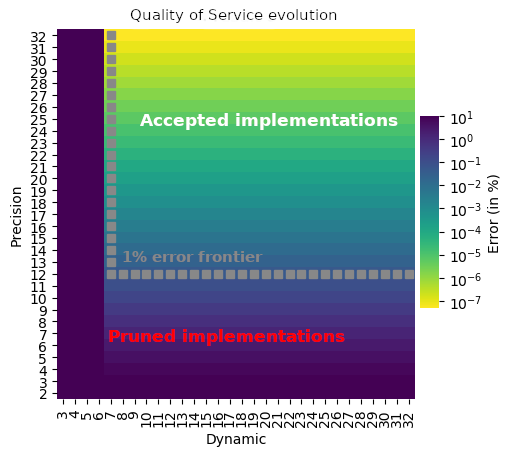
\includegraphics[width=1.0\textwidth]{Figures/results/quickPruning_annotated.png}
                \caption[Quick pruning of design space]{Quick pruning strategy for Quality of Service based exploration on\newline the dot product {\bf meta design}\textsuperscript{\styx} ({\it considering vectors of 8 elements})}
                \label{ch.expe:sec.strategies:ssec.qos:fig.quick}
            \end{figure}
        
            \begin{table}[ht!]
                \centering
                \begin{tabular}{cccc}
                    {\bf Optimization} & {\bf Simulated impl.} & {\bf Time} & {\bf Speed-up}\\
                    \hline
                    {\it Exhaustive pruning} & {\it 3844} & {\it 12m22s} & {\it ---}\\
                    \ccg Space reduction + & \ccg ~ & \ccg ~ & \ccg ~\\
                    \ccg exhaustive pruning & \ccg \multirow{-2}*{961} & \ccg \multirow{-2}*{03m07s} & \ccg \multirow{-2}*{$\times 3.97$}\\
                    Space reduction + & \multirow{2}*{255} & \multirow{2}*{05m03s} & \multirow{2}*{$\times 2.44$}\\
                    quick pruning (SeqSpace) & ~ & ~ & ~\\
                    \ccg Space reduction + & \ccg ~ & \ccg ~ & \ccg ~\\
                    \ccg quick pruning (MatrixSpace) & \ccg \multirow{-2}*{255} & \ccg \multirow{-2}*{00m49s} & \ccg \multirow{-2}*{$\times 15.14$}\\
                \end{tabular}
                \caption[Pruning results with respect to used optimizations]{Pruning results with respect to the used optimization on\newline the dot product {\bf meta design}\textsuperscript{\styx}}
                \label{ch.expe:sec.strategies:ssec.qos:table.quick}
            \end{table}

\clearpage
            We now consider the impact of both strategies and of the implementation details on the runtime.
            Table \ref{ch.expe:sec.strategies:ssec.qos:table.quick} exposes 4 different ways to prune the design space, that are based on the composition of three techniques:
            \begin{itemize}
                \item Space reduction --- \ie reducing the number of explored dimensions using the users knowledge about the parameters impact (Section \ref{ch.dse:sec.explorable:ssec.space})
                \item Strategy choice --- either the exhaustive or the quick pruning strategy% (Algo. \ref{ch.dse:sec.functional:ssec.basic:algo.quick})
                \item Space structure choice ---  either using a \lstinline{SeqSpace} or a \lstinline{MatrixSpace}
            \end{itemize}

            For all the considered techniques, we empirically checked that the resulting design spaces are identical, meaning that the same pruning is performed by those 4 techniques.
            The impact of the space reduction technique on the exploration time is obviously linear, as the number of estimated implementations is reduced in a linear way.
            In this context, as the {\it parallelism} parameter is not considered for \myAc{QoS}-based explorations, we reduce by a $\times 4$ factor the number of considered implementations (as this parameter can take 4 different values).
            Moreover, the number of implementations to simulate (column {\bf Simulated impl.} is also impacted by the chosen exploration strategy, as using the {\bf quick pruning} heuristic can lead to a relevant partition with less simulations to run, with respect to the {\bf exhaustive pruning} strategy.

            We can also remark that the performance of the {\bf quick pruning strategy} heavily relies on the chosen space structure: using a \lstinline{SeqSpace} representation, the quick pruning is actually slower than the exhaustive strategy, while using a \lstinline{MatrixSpace} results in a $\times 3.8$ $(= 15.14 / 3.97)$ speed-up, with respect to the strategy using both exhausting pruning and space reduction.

            We thus showed on this simple example that the {\bf quick pruning strategy} can be used to speed-up a \myAc{QoS}-based exploration strategy.
            Moreover, we provide further analysis about the \myAc{QoS} estimation and the quick pruning strategy in Appendix \ref{app.quick}.

\clearpage
        \subsection{Use Case: Exploring Black Scholes Designs}
        \label{ch.expe:sec.strategies:ssec.bs}
            We now consider a more realistic use case to demonstrate how the proposed methodologies can be leveraged to build a complex, application specific exploration strategy.
            To do so, we use a {\bf Black Scholes meta design} --- for which the implementation details are provided in Appendix \ref{app.benchmark} --- and define an iterative exploration strategy based on our expertise of \myAc{FPGA} design.

            As exposed in Appendix \ref{app.benchmark}, the {\bf meta design} exposes 5 parameters: the data representation parameters (\ie {\it dynamic} and {\it precision}), the number of iterations of the {\bf Monte Carlo} method, the number of parallel cores available, and the number of iterations of the {\bf Euler-Maruyama} method.

            \subsubsection{Defining the objectives of the exploration}
                The first thing to do to define an efficient exploration process is to clearly state the goal of the target flow.
                In this {\bf Black Scholes} based use case, we decided to try to \textbf{\emph{maximize the throughput of the generated accelerators, under the constraints that they fit on the target board and produce results with a controlled error rate}}.

                \begin{equation}
                    \label{ch.expe:sec.strategies:ssec.bs:eq.throughput}
                    T_{estimation.s^{-1}} = \frac{freq}{\Delta_c}
                \end{equation}

                \begin{equation}
                    \label{ch.expe:sec.strategies:ssec.bs:eq.latency}
                    \Delta_c \approx \frac{nbIter \times nbEuler}{nbCore}
                \end{equation}

                The throughput --- expressed in number of estimations by second --- can be approximated easily for these kernels, as they periodically produce a result: it is then computed as the ratio between the {\bf frequency} and the {\bf latency} of a given implementation (Eq. \ref{ch.expe:sec.strategies:ssec.bs:eq.throughput}).
                A theoretical latency (in number of cycles) --- \ie the (fixed) period between the production of each result --- can be computed using the Equation \ref{ch.expe:sec.strategies:ssec.bs:eq.latency}, as a huge majority of the computation cycles are spent in the {\bf Monte Carlo} cores iterations.%
                \footnote{This result has been verified empirically, proving that the impact of the control flow variations on the latency is negligible with respect to the actual computation cycles.}

                We also define an {\bf area} metric to verify that a design fits on the target board, using the maximum values of the usage percentage for the four considered metrics (\myAcs{LUT}, \myAcs{FF}, \myAcs{DSP} and \myAcs{BRAM}). 

            \subsubsection{Enhancing the design space}
                The next step to take in the introduced methodology is to instrument the {\bf meta design} with information on the metrics that will be used in the flow.

                \begin{figure}[ht!]
                    \begin{lstlisting}[xleftmargin=0mm,
                                       caption={[Expertise-based design space for Black Scholes meta design]Expertise-based design space for Black Scholes {\bf meta design}},
                                       label={ch.expe:sec.strategies:ssec.bs:list.bsSpace}]
class BlackScholes(
    @resource @qos @linear(8, 32)  dynamic: Int,
    @resource @qos @linear(8, 32)  precision: Int,
    @qos @pow2(5, 10)              nbIteration: Int,
    @qos @pow2(1, 6)               nbEuler: Int,
    @resource @pow2(2, 10)         nbCore: Int
) extends Module with Explorable\end{lstlisting}
                \vspace{-0.4cm}
                \end{figure}

                For this exploration, we will sequentially consider two concerns: a first stage will be based on the circuits \myAc{QoS}, and a second one will work over their resource usage.
                We hence need to define, for both of those metrics, which parameters have an impact on them, and which does not, based on our knowledge about the algorithm.
                The analysis to do so is introduced below, and is used to enhance the initial design space as exposed in Table \ref{app.benchmark:table.benchmark}, leading to the one introduced in Listing \ref{ch.expe:sec.strategies:ssec.bs:list.bsSpace}.

                Due to the probabilistic nature of the {\bf Monte Carlo} method, most of the exposed parameters have an impact on the \myAc{QoS}, either because they act on the data representation (as it is the case for both {\it precision} and {\it dynamic} parameters), or because they impact the number and the precision of the sampling in the Black Scholes equation (Eq. \ref{app.benchmark:sec.monteCarlo:eq.bsem}), as do the {\it number of iterations} and the {\it number of Euler-Maruyama iterations}.
                In contrast with these statements, the {\it number of cores} does not impact the circuits \myAc{QoS}, as it only modifies the temporal behaviour of the designs, and not their functionalities --- this parameter is hence not annotated as impacting the quality of service (using the \lstinline{@qos} annotation).

                As for the resource usage, we now try to identify which parameters impact the size of the generated designs.
                We can use our knowledge about the meta design structure to state that both {\it iteration parameters} (the global number of {\bf Monte Carlo} iterations, and the number of inner {\bf Euler-Maruyama} iterations) does not significantly impact the amount of resources used in a design.
                As a matter of fact, the number of iterations will act on the global latency of the design (Eq. \ref{ch.expe:sec.strategies:ssec.bs:eq.latency}), but will have a small impact on the resource usage, which mostly depends on the number of parallel cores and their size.%
                \footnote{The number of iterations actually impacts some counters in the control flow of the designs --- however, the impact is negligible with respect to the resources needed to implement the computation cores.}
                We thus annotate the data representation parameters and the {\it nbCore} parameter with \lstinline{@resource} to guide the exploration steps.

\clearpage
\vspace{-0.5cm}
            \subsubsection{Outlining the estimation transforms}
                Once the design space has been enhanced to guide the exploration, we need to define the different steps that are to be taken in the process.
                To build a compact definition of this exploration strategy, we define some helpers in Listings \ref{ch.expe:sec.strategies:ssec.bs:list.simu} and \ref{ch.expe:sec.strategies:ssec.bs:list.transforms} to build the transforms that are to be used in the flow.

                Listing \ref{ch.expe:sec.strategies:ssec.bs:list.simu} demonstrates how empirical \myAc{QoS} estimators can be integrated in \myAc{QECE}, in a condensed way.
                We define \lstinline{QualityOfService.simulation} as a transform calling the simulation backend to estimate the \myAc{RMSE} of a given implementation.
                The different {\bf generation parameters} of the simulated implementation are needed to instantiate the simulation test bench, and are thus retrieved from the {\bf point metrics} (the \lstinline{m} variable at line 1., which is used to define the parameters in lines 5-9).
                Moreover, some other parameters can be provided by the users when they are building such {\bf estimation transform} --- \eg in this use case, they provide the number of software iterations (line 10.) to compute the reference value for the {\bf Black Scholes} estimation, as well as the number of hardware simulations to run on each implementation to provide a significant result (line 11.).
                They also provide a {\it workload} (line 12.), which is the data distribution to be used in the test benches.

                \underline{Remark:} The circuits \myAc{QoS} are estimated using an empirical approach (Section \ref{ch.estimators:seq.qos:ssec.empirical}), as we use it to demonstrate the practicability of using the simulation backend in the estimation methodologies.
                However, one could also define an analytical formula to specify the relationship between the number of iterations of a given implementation on one hand, and the accuracy of the {\bf Black Scholes} approximation on the other.
                 While it would not be used to estimate the impact of the data representation over the \myAc{QoS}, it could allow to eliminate the parameters relative to the number of iterations from the design space, at least for the exploration steps that rely on simulations.

                As for Listing \ref{ch.expe:sec.strategies:ssec.bs:list.transforms}, it implements the analytical formulas from Equations \ref{ch.expe:sec.strategies:ssec.bs:eq.throughput} and \ref{ch.expe:sec.strategies:ssec.bs:eq.latency}.
                The transforms are easily defined, by specifying a pair $(n \rightarrow f: \{m_x, x \in [\![0, p]\!]\} \Rightarrow m_{x_{p+1}})$ with $n$ the name of the generated metric, and $f$ a function which operates on a set of metrics $\{m_x, x \in [\![0, p]\!]\}$ to generate a new metric named $n$ to be propagated in the exploration process.

                As can be seen in lines 1-4, the {\bf latency} is estimated in the {\bf pre-elaboration} stage (with respect to the \myAc{API} introduced in Section \ref{ch.estimators:sec.integration:ssec.api}), as it only relies on the generation parameters.

                On the other hand, both {\bf area} and {\bf throughput} are estimated in the {\bf post-elaboration} stage (lines 5-12).
                This is due to the fact that the \lstinline{Transforms.throughput} method is going to be called in the same exploration step that the synthesis flow:  as the formulas rely on the synthesis results, they must be computed after the elaboration process.

\clearpage
                The \lstinline{area} metric is computed by retrieving each resource percentage metric from the current implementation, using the maximal value to check if a design fits on the target board.
                To artificially eliminate the non fitting designs, we then use a temporary metric \lstinline{_throughput} to store the theoretical throughput as computed using Equation \ref{ch.expe:sec.strategies:ssec.bs:eq.throughput} (lines 8-9), but only assign it to the actual \lstinline{throughput} metric if the \lstinline{area} metric is under 100\% (lines 10-11).

\vspace{-0.4cm}
                \begin{figure}[h!]
                    \begin{lstlisting}[xleftmargin=0mm,
                                       basewidth={0.55em, 0.5em},
                                       caption={Defining an helper for empirical quality of service estimations},
                                       label={ch.expe:sec.strategies:ssec.bs:list.simu}]
object QualityOfService {
  val simulation = TransformSeq.simulation(m =>
    (                                                                       
      c =>                                                                                                        
        new BlackScholesTester(                                                                                   
          m("dynamic").toInt,                                                                                     
          m("precision").toInt,                                                                                   
          m("nbIteration").toInt,                                                                                 
          m("nbCore").toInt,                                                                                      
          m("nEuler").toInt,                                                         
          nbSoftIteration,                                                                                             
          nbSimulation,                                                                                                 
          workload                                                                                                
        )(c)                                                                                                      
      )                                                                                                           
    )                                                                                                            
}\end{lstlisting}
                \end{figure}
\vspace{-1.1cm}
                \begin{figure}[h!]
                    \begin{lstlisting}[xleftmargin=0mm,
                                       basewidth={0.55em,0.5em},
                                       caption={Transform helper for the exploration},
                                       label={ch.expe:sec.strategies:ssec.bs:list.transforms}]
object Transforms {
  val latency = TransformSeq.preElab(
    "latency" ->
      (m => (m("nbIteration") * m("nbEuler")) / m("nbCore"))
  )
  val throughput = TransformSeq.postElab(
    "area" ->
      (m => max(m("lut"), m("ff"), m("dsp"), m("mem"))),
    "_throughput" ->
      (m => m("freq") / m("latency")),
    "throughput" ->
      (m => if (m("area") > 1.0) 0.0 else m("_throughput"))
  )
}\end{lstlisting}
                \end{figure}

\clearpage
            \subsubsection{Defining the exploration strategy}
                After defining the transforms that are going to be used in the exploration process, the last step is to define the steps to be taken.
                We define a {\bf five steps} strategy for this use case, for which the code is exposed in Listing \ref{ch.expe:sec.strategies:ssec.bs:list.strategy}:
                \begin{enumerate}
                    \item \underline{\bf lines 1-5:} the design space is pruned for implementations that are estimated to induce an error of more than {\bf 5\%} (line 3.).

                        For this step, we use the {\bf quick pruning} algorithm (Algo. \ref{ch.dse:sec.functional:ssec.basic:algo.quick}) to quickly partition the space in this pruning step (line 1.).
                        Moreover, as we only consider the \myAc{QoS} of the different implementations, we specify that the framework can eliminate all the dimensions that are not annotated with \lstinline{@qos} (line 4.).
                        Indeed, we use the \lstinline{QualityOfService.simulation} transform from Listing \ref{ch.expe:sec.strategies:ssec.bs:list.simu} to compute the \myAc{QoS} (line 2.).
                    \item \underline{\bf line 6:} this line specifies how we reduce the dimensions of the design space for the remaining exploration steps.
                        All the {\bf meta design parameters} (see Fig. \ref{ch.expe:sec.strategies:ssec.bs:list.bsSpace}) that are not annotated with \lstinline{@resource} do no act on the resource metrics, and are thus removed from the dimensions. 
                        They are in fact the parameters acting on the number of iterations: {\it nbIteration} and {\it nbEuler}.
                        Actually, we can state two things at this point: all the remaining designs are acceptable with respect to the needed \myAc{QoS} in this use case, and reducing the number of iterations can only benefit to improve both the resource usage and the throughput.%
                        \footnote{Increasing the number of iterations can only improve the \myAc{QoS} at the cost of {\bf latency} increase (Eq. \ref{ch.expe:sec.strategies:ssec.bs:eq.latency}), yet we already have a sufficiently low error after the pruning step.}

                        The boolean parameter of the \lstinline{context.reduceDimension} method specifies that the dimension removal will project the parameters on the {\bf minimal values} in the space --- as we want to keep the number of iterations as low as possible among the remaining designs.

                        By removing those two dimensions from the design space, the number of remaining implementations is hence heavily reduced.%, which allows to speed-up the process.
                    \item \underline{\bf line 7:} we compute the latency of each remaining implementation.
                    \item \underline{\bf lines 8-12:} we select the "minimal point" of the remaining design space (the point with the minimal sum of parameters) and put it in front of the design space, as the next step will use it as a starting point.
                    \item \underline{\bf lines 13-17:} we use a {\bf gradient descent} algorithm to find a local optimum with respect to the objective of the exploration.

                        In this step, we run syntheses in order to provide a realistic estimation of both resource usage and operating frequency, and it is thus necessary to adopt a clever strategy to limit the number of costly process runs.
                        We hence use neighbourhood explorations to iteratively find an acceptable solution to the users.
                \end{enumerate}

                \begin{figure}[h!]
                    \begin{lstlisting}[xleftmargin=0mm,
                                       basewidth={0.55em, 0.5em},
                                       caption={[Black Scholes exploration strategy]Expertise-based exploration strategy for Black Scholes\newline implementations},
                                       label={ch.expe:sec.strategies:ssec.bs:list.strategy}]
val strategy = context.buildStrategy(                                                                                    
  context.quickPrune[BlackScholes](                                                                             
    QualityOfService.simulation,
    _.error > 0.05,                                                                                            
    metric = Some(new qos)                                                                              
  ),                                                                                                                
  context.reduceDimension[BlackScholes](new resource, true),                                                    
  context.map[BlackScholes](Transforms.latency),                                                     
  context.sort[BlackScholes](                                                                                   
    TransformSeq.empty,                                                                                           
    m => m("dynamic") + m("precision") + m("nbCore"),                                                                 
    (_ < _)                                                                                                           
  ),                                                                                                                  
  context.gradient[BlackScholes](                                                                               
    TransformSeq.synthesis ++ Transforms.throughput
    func = _("throughput"),                                                                                           
    cmp = (_ > _)  
  )                                    
)\end{lstlisting}
                \end{figure}

                We hence defined a complex, expertise-based exploration strategy which takes the best of the users knowledge to guide the framework and to speed-up the traversal process.
                In order to provide an analysis on the relevance of such strategies, we ran multiple exploration processes to expose the interests of the {\bf meta exploration} choices that led to the definition of Listing \ref{ch.expe:sec.strategies:ssec.bs:list.strategy}.
                
        \subsection{Results of the Black Scholes Exploration}
        \label{ch.expe:sec.strategies:ssec.results}
            In this last section, we will analyse the results of the exploration strategy defined for the Black Scholes use case, to exhibit the advantages of defining a custom strategy in a functional fashion.

\clearpage
            \subsubsection{Comparing the pruning strategies}
                A first analysis can be done about the quality of the pruning processes, by comparing the {\bf exhaustive pruning} and the {\bf quick pruning} strategies on the Black Scholes use case.

                % \tdf{quality of service pruning + venn fiagramm}
                \begin{table}[ht!]
                    \begin{tabular}{ccccc}
                        {\bf Error} & {\bf Number} & \multirow{2}*{{\bf Strategy}} & {\bf Exploration} & \multirow{2}*{{\bf Speed-up}} \\
                        {\bf threshold} & {\bf of impl.} & ~ & {\bf time} & ~ \\
                        \hline
                        \ccg ~ & \ccg ~ & \ccg Exhaustive pruning & \ccg 46h29m19s & \ccg - \\
                        \multirow{-2}*{\ccg 5\%} & \multirow{-2}*{\ccg 202500} & \ccg Quick pruning & \ccg 32h59m29s & \ccg $\times 1.40$ \\
                        \multirow{2}*{2\%} & \multirow{2}*{202500} & Exhaustive pruning & 46h21m42s & - \\
                        ~ & ~ & Quick pruning & 48h46m53s & \inred{$\times 0.95$}
                    \end{tabular}
                    \caption[Comparing pruning strategies on Black Scholes]{Comparing the pruning strategies over Black Scholes kernels\textsuperscript{\styx}}
                    \label{ch.expe:sec.strategies:ssec.bs:table.qor}
                \end{table}

                \begin{figure}[h!]
                    % \centering
                    \begin{subfigure}{0.49\textwidth}
                        \centering
                        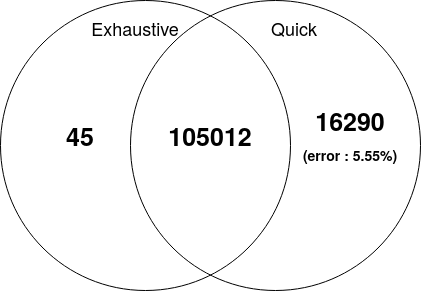
\includegraphics[width=1.0\textwidth]{Figures/results/qor-venn-5}
                        \caption{5\% error threshold}
                        \label{ch.expe:sec.strategies:ssec.bs:fig.venn:sfig.5}
                    \end{subfigure}
                    ~
                    \begin{subfigure}{0.49\textwidth}
                        \centering
                        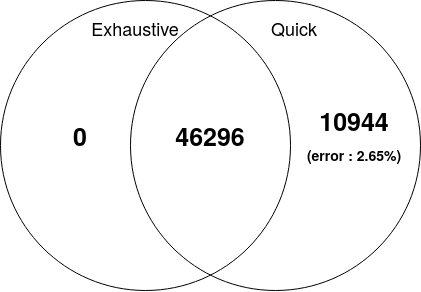
\includegraphics[width=1.0\textwidth]{Figures/results/qor-venn-2}
                        \caption{2\% error threshold}
                        \label{ch.expe:sec.strategies:ssec.bs:fig.venn:sfig.2}
                    \end{subfigure}
                    \caption[Comparing the accuracy of the pruning strategies]{Comparing the accuracy of the pruning strategies on Black Scholes\textsuperscript{\styx}}
                    \label{ch.expe:sec.strategies:ssec.bs:fig.venn}
                \end{figure}

                Table \ref{ch.expe:sec.strategies:ssec.bs:table.qor} introduces the results of four different explorations processes, to compare both strategies using two different {\bf error thresholds} for the pruning.
                In those experiments, only the pruning step (lines 1-5 in Listing \ref{ch.expe:sec.strategies:ssec.bs:list.strategy}, compared to an exhaustive version of it) is considered, and we compare the remaining implementations in Figure \ref{ch.expe:sec.strategies:ssec.bs:fig.venn}.

                As we can see in the table, depending on the error threshold, the {\bf quick pruning strategy} can lead to a faster pruning of the space (as it is the case with a 5\% threshold), or a slower one if the frontier is difficult to estimate and requires a lot of neighbourhood exploration steps to do so.

                We can also see in Figure \ref{ch.expe:sec.strategies:ssec.bs:fig.venn} that the quick pruning heuristic is not perfect: %
                for example, using an acceptable error rate of 5\% (Fig. \ref{ch.expe:sec.strategies:ssec.bs:fig.venn:sfig.5}), {\bf 105012 remaining implementations} were common to both strategies, while {\bf 45} were pruned by the quick strategy and not by the exhaustive one, and {\bf 16290} were pruned by the exhaustive strategy, and not by the quick one (on a total of {\bf 202500 different implementations}).
                If we consider the exhaustive pruning to be the baseline --- as estimating the \myAc{QoS} of each implementation leads to a more realistic pruning of the design space, even if the empirical approach can induce erroneous data --- we can remark that the quick pruning strategy tends to prune less implementations that the exhaustive one.

                This shows that this strategy can lead to erroneous choice from the exploration tools --- however, the average errors in the designs that should have been pruned by the quick heuristic but were not are also displayed in Figures \ref{ch.expe:sec.strategies:ssec.bs:fig.venn:sfig.5} and \ref{ch.expe:sec.strategies:ssec.bs:fig.venn:sfig.2} (with average errors of respectively 5.55\% and 2.65\%).
                These errors are computed on the points that were estimated in the frontier building algorithms, through the neighbourhood exploration: those implementations are thus near to this limit, and this is why they are not pruned as they would have been in an exhaustive process.

                \underline{Remark:} among those points, some errors are approximated instead of being estimated, in order to keep the number of simulations low.
                This is done on the points that are considered "above" the built frontier, but that were not considered in the neighbourhood exploration process used to build this frontier.
                In order to produce an error metric anyway, even if not actual \myAc{QoS} estimation is performed, an artificial metric is built by copying the error value of one of the points on the frontier to add it to every point that was not estimated in frontier construction process.
                This means that the average {\bf error} values introduced in Figure \ref{ch.expe:sec.strategies:ssec.bs:fig.venn} relies on this approximation, and should be considered carefully.

\vspace{-0.1cm}
            \subsubsection{Exploiting a complex strategy for exploration}
                We now consider a full exploration process based on the strategy exposed in Listing \ref{ch.expe:sec.strategies:ssec.bs:list.strategy}, to demonstrate the usability of \myAc{QECE} on a complex use case.
                                
                \begin{table}[h!]
                    \scalebox{0.9}{
                        \hspace{-0.5cm}
                        \begin{tabular}{c|ccc|cc|c}
                            \multirow{2}*{{\bf Rank}} & \multirow{2}*{{\bf Parameters}} & \multirow{2}*{{\bf Error}} & {\bf Throughput} & \multicolumn{2}{c}{{\bf Area}} & \multirow{2}*{{\bf Frequency}} \\
                            ~ & ~ & ~ & ($est.s^{-1}$) & Max \% & Resource & ~ \\
                            \hline
                            \ccg 1 & \ccg [12, 21, 64, 2, 64] & \ccg 5.34\% & \ccg 125.06 & \ccg 25\% & \ccg \myAc{DSP} & \ccg 250.13 MHz \\
                            2 & [12, 20, 64, 2, 64] & 4.6\% & 125.06 & 25\% & \myAc{DSP} & 250.13 MHz \\
                            \ccg 3 & \ccg [12, 22, 64, 2, 64] & \ccg 6.54\% & \ccg 125.03 & \ccg 25\% & \ccg \myAc{DSP} & \ccg 250.06 MHz \\
                            4 & [13, 21, 64, 2, 64] & 6.06\% & 125.03 & 25\% & \myAc{DSP} & 250.06 MHz \\
                            \ccg 5 & \ccg [12, 22, 64, 2, 32] & \ccg 5.34\% & \ccg 62.53 & \ccg 12.5\% & \ccg \myAc{DSP} & \ccg 250.13 MHz \\
                        \end{tabular}
                    }
                    \caption[Exploration results on Black Scholes]{Best implementations found using the exploration strategy from Listing \ref{ch.expe:sec.strategies:ssec.bs:list.strategy}\textsuperscript{\styx}. The whole exploration process took approximatively 38 hours to synthesize the 27 more interesting candidate implementations --- through a gradient-based approach --- and sort them.}
                    \label{ch.expe:sec.strategies:ssec.bs:table.results}
                \end{table}

\vspace{-0.15cm}
                Table \ref{ch.expe:sec.strategies:ssec.bs:table.results} introduces the five best implementations found at the end of the exploration process --- after 37 hours and 47 minutes.
                The {\bf parameters} are compressed in the table, and correspond respectively to the {\bf dynamic}, the {\bf precision}, the {\bf number of iterations}, the {\bf number of Euler-Maruyama iterations} and the {\bf number of cores}.
                A total of 27 different implementations have been considered in the last step of the process, which we will denote as being the {\bf synthesis step}.
                
                The first thing we can remark is that the pruning criteria is not strictly respected, as was shown in the previous section --- however, the error overhead can be considered acceptable for some use cases, as it barely reaches 30\% of the target error threshold.
                
                We can also see that the four best implementations use 64 parallel cores, resulting in a resource usage of $1/4$ of the target board, and achieving a throughput of 125 estimations by second.                

                One could thus argue that we could use up to 256 parallel cores, to fill the targeted \myAc{FPGA}.
                However, after the pruning step, we found that 64 iterations (with 2 Euler-Maruyama inner iterations) were enough to ensure a satisfying \myAc{QoS} on the implementations shown in the table.
                As the number of cores cannot be larger than the number of iterations by design --- it is an inner constraint of the Black Scholes meta design used in this use case, and could be addressed by modifying the \chisel{} description --- the gradient algorithm did not fully explore the {\bf number of core} dimension, resulting in a sub optimal solution.
                Nevertheless, as the kernels are independent, this exploration showed that we could fit {\bf four Black Scholes accelerators} in parallel on the target board, using the resulting generation parameters.

                As for the temporal behaviour of this experiment, we cannot expose a baseline similar to the previous ones, as an exhaustive exploration of the remaining design space would be too long (approximatively 6000 different implementations to synthesize, which would take up to 500 days to complete, with respect to the 2 hours timeout used).

                However, we could cope with this problem by using a more hierarchical approach to build the baseline.
                For example, some approaches in the literature uses a preliminary {\bf random sampling} to identify {\bf regions of interest} in the design space, \ie sub spaces where the solutions are expected to be the best ones \cite{awais_ldax_2021}.
                This strategy could be leveraged for two usages in our experiment.
                First of all, we could use partial sampling of the design space to run syntheses and state if the local approach of the gradient algorithm caused a sup optimal choice in the space.
                Moreover, we could also use such sampling to select the starting point of the gradient descent, instead of arbitrarily selecting a point as it was done (lines 8-12 of Listing \ref{ch.expe:sec.strategies:ssec.bs:list.strategy}).


%%%%%%%%%%%%%%%%%%%%%%%%%%%%%%%%%%%%%%%%%%%%%%%%%%%%%%%%%%%%%%%%%%%%%%%%%%%%%%%%%

\clearpage
% SECTION
\section{Synthesis on the Experiments}
\label{ch.expe:sec.synthesis}
\vspace{-0.08cm}
    \subsubsection{Experimental contributions}
\vspace{-0.04cm}
        In this chapter, we exposed the implementation details of a software demonstrator (named \myLongAc{QECE}{Quick Exploration using Chisel Estimators}) for the design methodologies that have been introduced in Chapters \ref{ch.estimators} and \ref{ch.dse}.
        Doing so, we built a generic and modular framework for \myLongAc{DSE}{Design Space Exploration} processes targeting \myLongAcs{FPGA}{Field-Programmable Gate Array}.

        We also introduced a benchmark of algorithms that are representative of the usage of \myAcs{FPGA} as hardware accelerators, in order to demonstrate the usability of \myAc{QECE} in realistic use cases.
        
        We finally ran multiple explorations as experiments to analyse the advantages and the limitations of both our methodologies and our framework over the hardware development processes.
        We explored the design spaces of three different {\bf meta designs} --- \myLongAc{GEMM}{General Matrix Multiply}, \myLongAc{FFT}{Fast Fourier Transform} and Black Scholes --- and considered different objectives and constraints to show that one can define custom strategies for their exploration processes, based on their expertise about both the algorithm being implemented and the \myAc{FPGA} board being targeted.
    
\vspace{-0.08cm}
    \subsubsection{Synthesis on the results}
\vspace{-0.04cm}
        In order to demonstrate how one can leverage its expertise about both the application being explored and the \myAc{FPGA} board being targeted, we considered two different types of objectives to be considered at exploration time.

        To begin with, we used both \myAc{GEMM} and \myAc{FFT} {\bf meta designs} to expose how a high level estimation of the resource usage can lead to the building of efficient exploration strategies, and demonstrated that such strategies can lead to speeding up exploration processes by a significant factor, reducing the exploration time from 13 hours to 4 hours only for \myAc{GEMM}.

        We then used a {\bf Monte Carlo} based design, the {\bf Black Scholes} pricing {\bf meta design}, to show how one can consider the \myLongAc{QoS}{Quality of Service} of the developed circuits to build strategies that sequentially consider different metrics to optimize.
        We implemented a pruning heuristic that can be used to more or less efficiently partition a design space without having to simulate exhaustively the implementations that compose it, with speed-ups up to 40\% with respect to the exhaustive strategy, and exposed a complex, expertise based {\bf meta exploration strategy} that can be used to find efficient architectures for the given use case.
        Doing so, the number of implementations to synthesize is heavily reduced, and only 27 different designs are considered in those long processes, in a total design space of approximatively 6000 different circuits, where an exhaustive exploration is indeed impracticable.
    
    \subsubsection{Discussion on the approach}
        While we did show that exhibiting an expertise based strategy --- that uses custom defined metrics and estimation methodologies --- can lead to a quicker convergence of the exploration processes toward an acceptable solution (if not an optimal one), we also showed that an inadequate strategy can lead to suboptimal solutions, and can take more time that the standard exploration flows that rely on heavy synthesis tools.
        The strategies that are being compared here are quite naive and simple, and \myAc{QECE} would greatly benefit of the implementation of more advanced heuristics, in order to provide users with a more furnished library of configurable exploration steps.

        However, we demonstrated the practicability of a novel way to consider the exploration processes, using the functional programming feature to define such flows in a concise yet intelligible way for the users, by considering an exploration process as a succession of basic steps.
        We also exhibited the interests of the emerging \myLongAc{HCL}{Hardware Construction Language} paradigm for hardware development, proving that a potentially consequent overhead on the {\it a priori} analysis of the algorithm can lead to reusable hardware generators, which can then be easily adapted to new use cases.

%%%%%%%%%%%%%%%%%%%%%%%%%%%%%%%%%%%%%%%%%%%%%%%%%%%%%%%%%%%%%%%%%%%%%%%%%%%%%%%%%
 %%%%%%%%%%%%%%%%%%%%%%%%%%%%%%%%%%%%%%%%%%%%%%%%%%%%%%%%%%%%%%%%%%%%%%%%%%%%%%%
